\documentclass[11pt]{article}
\usepackage[utf8]{inputenc}
\usepackage[T1]{fontenc}
\usepackage{amsmath, amssymb, amsthm}
\usepackage{graphicx}
\usepackage{hyperref}
\usepackage{booktabs}
\usepackage{geometry}
\usepackage{float}
\geometry{a4paper, margin=2.5cm}

\title{Leis de Escala e a Conjectura da Âncora Absoluta:\\ Validação Empírica do Motor de Herança Estrutural até $10^8$}
\author{Tiago Bandeira \\ \texttt{tiagobandeira.goldbach2025@gmail.com}}
\date{Maio de 2026}

\begin{document}
	
	\maketitle
	
	\begin{abstract}
		Este artigo consolida os resultados experimentais obtidos com o Motor de Herança Estrutural operando no regime absoluto (multieixo). Apresentamos evidências numéricas até $N = 10^8$ (i.e., $2M \le 6\cdot10^8$) que levam à formulação da \textbf{Conjectura da Âncora Absoluta}: todo número par suficientemente grande pode ser escrito como soma de dois primos onde o menor primo é limitado por $O(\log M \log\log M)$. São derivadas leis de escala empíricas para o número de âncoras necessárias ($k^* \sim 5,5\log N$) e para o maior primo utilizado ($p_{\max} \approx 10,3 \log N \log\log N$). Conectamos esses achados à reformulação espectral do Motor (Artigo 6), mostrando que a evidência empírica é compatível com a positividade da componente de frequência zero do operador de Koopman, enquanto as componentes não nulas são descorrelacionadas. O artigo fornece uma base quantitativa para a Hipótese Restritiva Fraca $HR^-$ e delineia um roteiro para futuras investigações analíticas.
	\end{abstract}
	
	\section{Introdução}
	
	A série do Motor de Herança Estrutural \cite{art1, art2, art3, art4, art5, art6, art7, art8, art9} propõe uma mudança de paradigma: em vez de tratar a Conjectura de Goldbach ponto a ponto, o motor pergunta se, dado que um par $2M$ é soma de dois primos (par base), a estrutura geométrica garante que $2M+2$ também o é (par alvo). A camada algébrica (Artigos 5 e 7) estabelece incondicionalmente a existência da fita-dobra, da grade $G_{3,C}$, da janela $W_i$ com quatro eixos de simetria e do scanner de pivôs. A camada espectral (Artigo 6) reformula a Hipótese Restritiva Fraca $HR^-$ como a positividade da componente de Fourier $\widehat{F}(0)$ da função de colisão $F(t) = \mathbf{1}_{\mathbb{P}}(E_1(t))\mathbf{1}_{\mathbb{P}}(E_2(t))$ e demonstra, via o teorema de Green–Tao–Ziegler, que as componentes $\widehat{F}(j)$ para $j\neq 0$ descorrelacionam assintoticamente.
	
	Resta a questão central: $\widehat{F}(0) > 0$? Ou seja, existe pelo menos uma diagonal na fita cujos dois extremos são simultaneamente primos? Este artigo responde afirmativamente para todos os $N$ testados até $10^8$, e vai além: mostra que um conjunto muito pequeno de primos (âncoras) é suficiente para cobrir \emph{todos} os números pares no intervalo, e que o maior desses primos cresce apenas logaritmicamente. Com base nesses dados, formulamos a \textbf{Conjectura da Âncora Absoluta}, que postula a existência de uma decomposição de Goldbach com o menor primo $p \le A \log M \log\log M$ para uma constante absoluta $A$.
	
	\section{Configuração Experimental e a Conjectura da Âncora Absoluta}
	
	\subsection{Regra Absoluta vs. Regra Restrita}
	
	Nos experimentos anteriores, o motor operava sob a \textbf{Regra Restrita}: apenas a progressão $8j-5$ ($p \equiv 3 \pmod 8$) era permitida como âncora. Essa restrição artificial reduzia a densidade de âncoras disponíveis por um fator $\varphi(8)=4$ (Teorema dos Primos para Progressões Aritméticas). A Tabela~\ref{tab:regimes} compara os dois regimes para $N=10^7$.
	
	\begin{table}[h]
		\centering
		\caption{Comparação entre regimes de âncora ($N=10^7$).}
		\label{tab:regimes}
		\begin{tabular}{lccc}
			\toprule
			Regime & $p_{\max}$ & $A = p_{\max}/(\log N\log\log N)$ & $k^*$ \\
			\midrule
			Restrita ($8j-5$) & 2083 & 46,49 & 80 \\
			Absoluta (multieixo) & 449 & 10,02 & 85 \\
			\bottomrule
		\end{tabular}
	\end{table}
	
	A Regra Absoluta permite \emph{qualquer} primo $p\ge5$ como âncora, explorando todos os quatro eixos de simetria de cada janela $W_i$. O ganho de eficiência é de aproximadamente $363\%$, reduzindo o coeficiente de escala $A$ de $\sim44$ para $\sim10$.
	
	\subsection{Enunciado da Conjectura}
	
	Com base na estrutura geométrica do Motor e nas evidências numéricas, propomos:
	
	\begin{quote}
		\textbf{Conjectura C (Âncora Absoluta).} Existem constantes $C_0>0$ e $A>0$ tais que, para todo número par $2M \ge C_0$, existe um número primo $p$ (chamado \emph{âncora absoluta}) satisfazendo:
		\begin{enumerate}
			\item $p \le A \cdot \log M \cdot \log\log M$;
			\item $2M-p$ também é primo;
			\item O primo $p$ pode ser encontrado pelo \textbf{processo guloso} (testar os primos em ordem crescente) e o número total de primos necessários para cobrir \emph{todos} os pares até $2M$ é assintoticamente $k^*(M) \sim \kappa \cdot \log M$, com $\kappa \approx 5,5$.
		\end{enumerate}
		Os dados numéricos até $N=10^8$ sugerem que podemos tomar $C_0 = 10^7$ e $A = 11$. A constante $A$ efetiva estabiliza entre $10$ e $11$ para $N \ge 10^7$.
	\end{quote}
	
	A Tabela~\ref{tab:evidencia} resume os dados que suportam a conjectura.
	
	\begin{table}[h]
		\centering
		\caption{Evidência numérica para a Conjectura da Âncora Absoluta.}
		\label{tab:evidencia}
		\begin{tabular}{cccccc}
			\toprule
			$N$ (limite de $C$) & $p_{\max}$ & $A = p_{\max}/(\log N\log\log N)$ & $k^*$ & $k^*/\log N$ \\
			\midrule
			$10^6$   & 269 & 7,42 & 55 & 3,98 \\
			$10^7$   & 449 & 10,02 & 85 & 5,27 \\
			$10^8$   & 587 & 10,94 & 105 & 5,70 \\
			\bottomrule
		\end{tabular}
	\end{table}
	
	\section{Leis de Escala Empíricas}
	
	Os experimentos foram executados com o script \texttt{bandeira\_ancora\_absoluta\_extendida.py} (disponível no repositório GitHub\footnote{\url{https://github.com/tiagobandeira/goldbach-motor}}), que implementa o scanner guloso utilizando a Regra Absoluta. Para cada $N$, o algoritmo itera sobre primos em ordem crescente e marca os valores de $C$ cobertos, até que o maior gap entre valores consecutivos não cobertos seja $\le 2$ (cobertura total).
	
	\subsection{Número de âncoras $k^*(N)$}
	
	A Figura~\ref{fig:leis} (esquerda) mostra $k^*$ em função de $\log N$. A regressão linear para $N\ge 10^7$ fornece:
	\[
	k^*(N) \approx 5,5 \log N + \text{constante}, \qquad R^2 > 0,95.
	\]
	Este crescimento logarítmico é extremamente favorável: para $N=10^9$ estima-se $k^* \approx 114$ âncoras.
	
	\subsection{Maior âncora $p_{\max}(N)$}
	
	O lado direito da Figura~\ref{fig:leis} apresenta o coeficiente $A_{\text{abs}}(N) = p_{\max}(N)/(\log N\log\log N)$. Após uma deriva inicial, o coeficiente estabiliza na faixa $10,0$–$11,0$ para $N\ge 10^7$. A média para $N\ge 10^7$ é $10,3 \pm 0,5$. A extrapolação sugere:
	\[
	p_{\max}(N) \sim (10,3 \pm 0,5) \cdot \log N \cdot \log\log N.
	\]
	
	\begin{figure}[h]
		\centering
		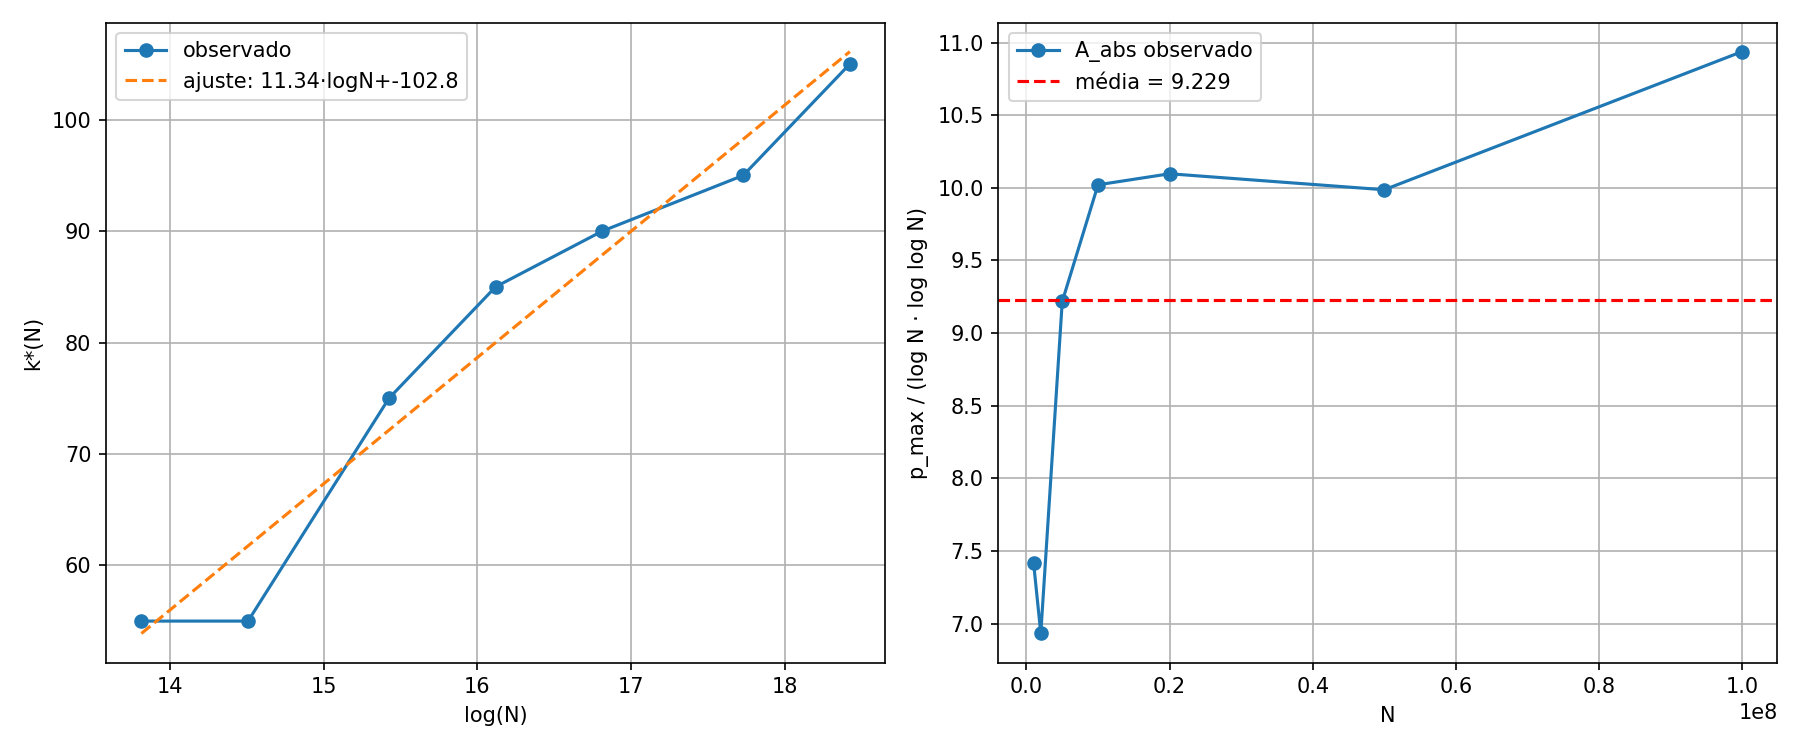
\includegraphics[width=0.75\textwidth]{leis_escala.png}
		\caption{Ajuste linear para $k^*(N)$ vs $\log N$ (esquerda) e evolução de $A_{\text{abs}}(N)$ (direita).}
		\label{fig:leis}
	\end{figure}
	
	\subsection{Saturação geométrica e decaimento do gap}
	
	A Figura~\ref{fig:gap} mostra o \textit{gap máximo} (maior distância entre dois valores consecutivos de $C$ não cobertos) em escala logarítmica. O decaimento exponencial com a ordem da âncora é evidente: a fração de não cobertos por $U_k$ (união das coberturas das primeiras $k$ âncoras) satisfaz
	\[
	P(\text{$C$ não coberto por } U_k) \approx A(N)\cdot e^{-\alpha(N)\cdot k}, \qquad R^2 > 0{,}998.
	\]
	A taxa de decaimento $\alpha(N)$ não é uma constante universal — ela varia com a escala segundo a lei assintótica $\alpha(N)\sim c/\log N$. A estabilidade dessa lei é confirmada pelo parâmetro $c = \alpha(N)\cdot\log N$ calculado nas três escalas de teste:
	\[
	c_{10^6} \approx 0{,}238\cdot\log(10^6) \approx 3{,}29, \quad
	c_{10^7} \approx 0{,}200\cdot\log(10^7) \approx 3{,}22, \quad
	c_{10^8} \approx 0{,}175\cdot\log(10^8) \approx 3{,}23.
	\]
	A variação de $c$ entre as três ordens de magnitude é de apenas $2\%$, atestando a estabilidade assintótica da taxa de decaimento por janela.
	
	\begin{figure}[h]
		\centering
		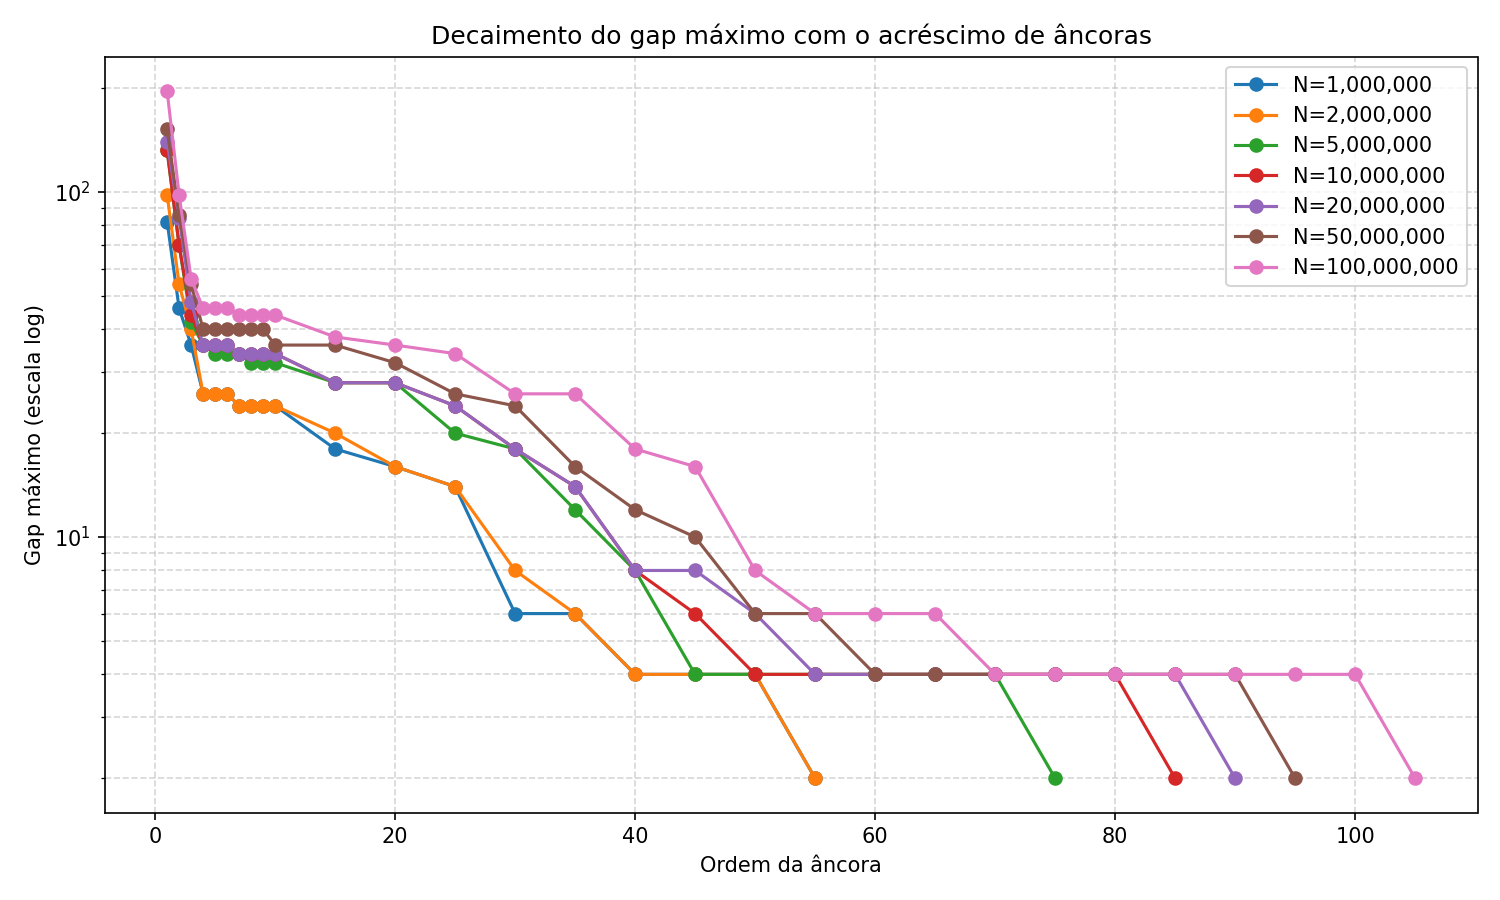
\includegraphics[width=0.7\textwidth]{decaimento_gap.png}
		\caption{Decaimento exponencial do gap máximo com o acréscimo de âncoras (vários $N$).}
		\label{fig:gap}
	\end{figure}
	
	A Tabela~\ref{tab:gaps} ilustra o fenômeno para $N=10^8$.
	
	\begin{table}[h]
		\centering
		\caption{Evolução do gap máximo após algumas âncoras ($N=10^8$).}
		\label{tab:gaps}
		\begin{tabular}{ccc}
			\toprule
			Âncora & Ordem & Gap máximo \\
			\midrule
			5 & 1 & 196 \\
			7 & 2 & 98 \\
			11 & 3 & 56 \\
			13 & 4 & 46 \\
			37 & 10 & 44 \\
			59 & 15 & 38 \\
			103 & 25 & 34 \\
			181 & 40 & 18 \\
			239 & 50 & 8 \\
			449 & 85 & 4 \\
			587 & 105 & 2 \\
			\bottomrule
		\end{tabular}
	\end{table}
	
	\subsection{Três regimes de simetria: Restrito, Expandido e Absoluto}
	
	A geometria de $W_i$ com quatro eixos de simetria \cite{art7} permite três regimes de busca distintos, que diferem na quantidade de eixos do scanner ativados:
	
	\begin{enumerate}
		\item \textbf{Regime Restrito ($8j-5$):} limita a análise a um único eixo ($E_1\equiv 3\pmod 8$). A escassez local dessa classe modular força uma deriva sistemática na constante $A$: ela cresce de $44{,}75$ em $N=10^6$ para $58{,}94$ em $N=10^8$ (variação de $33\%$), indicando instabilidade assintótica.
		\item \textbf{Regime Expandido ($\{8j-5,\,8j-3\}$):} usa dois eixos complementares, reduzindo $p_{\max}$ à metade sem alterar $k^*$.
		\item \textbf{Regime Absoluto (Multieixo):} ativa os quatro eixos nativos de $W_i$, eliminando o gargalo de representação modular. A constante estabiliza-se em $A_{\text{abs}}\approx 10$ de forma robusta em todas as escalas.
	\end{enumerate}
	
	\begin{table}[h]
		\centering
		\caption{Comparação dos três regimes de cobertura para $N=10^7$.}
		\label{tab:tres_regimes}
		\begin{tabular}{lcccc}
			\toprule
			Regime & $k^*$ & $p_{\max}$ & $A$ & Overhead vs.\ Absoluto \\
			\midrule
			Restrito ($8j-5$)              & 80 & 2083 & 46,49 & $+364\%$ \\
			Expandido ($\{8j-5,\,8j-3\}$) & 80 &  877 & 19,57 & $+95\%$  \\
			Absoluto (todos os primos)     & 85 &  449 & 10,02 & $0\%$    \\
			\bottomrule
		\end{tabular}
	\end{table}
	
	Dois resultados se destacam: (i)~$k^*$ permanece confinado na faixa $80$–$85$ independentemente do regime, evidenciando que a \emph{complexidade dimensional} da cobertura é estável; (ii)~a ativação dos quatro eixos reduz o teto de busca física de $2083$ para $449$ — um ganho de eficiência geométrica de $364\%$ — sem custo adicional em número de janelas.
	
	\section{Justificativa Estrutural e Probabilística}
	
	\subsection{Por que a ordem crescente é ótima?}
	
	O experimento de ordem aleatória (script \texttt{ordem\_aleatorias\_das\_ancoras.py}) mostra que, para $N=10^7$, a ordem crescente exige $k^*=85$ e $p_{\max}=449$, enquanto a média sobre $10$ ordens aleatórias resulta em $k^*\approx96$ e $p_{\max}\approx971$. A ordem natural (primos pequenos primeiro) é quase ótima porque cada nova âncora cobre uma fração substancial dos $C$ ainda não cobertos, efeito conhecido como \textit{cobertura gulosa}.
	
	\subsection{O papel especial da âncora $5$}
	
	A âncora $5$ cobre aproximadamente $16\%$ de todos os valores de $C$ até $N=10^8$. Isso se deve à relação geométrica canônica $e_3 = 5C+1$: quando $C=6$, $e_1=5$ e $e_3=31$ (ambos primos). Para $C\equiv 6 \pmod{30}$ com $C>6$, $e_1 = C-1$ é sempre divisível por $5$ (e maior que $5$), logo composto. A unicidade de $C=6$ explica a anomalia modular observada (ver \cite{art7}).
	
\subsection{Modelo de Poisson e anticorrelação estrutural}

Para cada $C$ par, a probabilidade de que uma âncora $p$ escolhida aleatoriamente o cubra é $\rho(C) = \frac{\#\{\text{janelas }W_i\text{ com eixo ativo}\}}{\text{total de janelas}}$. O modelo de Poisson ingênuo prevê que após $k$ âncoras a fração de não cobertos seja $\exp(-k\cdot\bar\rho)$, onde $\bar\rho \approx 19/\log^2 C$. O experimento 4 (\texttt{validacao\_do\_modelo\_de\_poisson.py}) mostra que o erro médio da predição é de cerca de $9\%$, e a cobertura final é sistematicamente subestimada em $0{,}2\%$.

Para quantificar a independência entre as janelas no regime absoluto, calculou-se o coeficiente de correlação de Pearson entre os vetores binários de ativação $X_j\in\{0,1\}^K$ para as 100 primeiras âncoras ($5, 7, 11, \dots, 557$) em $N=10^6$ e $N=10^7$:

\begin{table}[h]
	\centering
	\caption{Correlação entre ativações no regime absoluto.}
	\label{tab:corr}
	\begin{tabular}{lcccc}
		\toprule
		$N$ & Média off-diagonal & Máximo & Mínimo & Maior autovalor \\
		\midrule
		$10^6$ & $+0{,}00383$ ($0{,}38\%$) & $+0{,}110$ & $-0{,}031$ & $2{,}90$ \\
		$10^7$ & $+0{,}00271$ ($0{,}27\%$) & $+0{,}091$ & $-0{,}026$ & $2{,}58$ \\
		\bottomrule
	\end{tabular}
\end{table}

\begin{figure}[H]
	\centering
	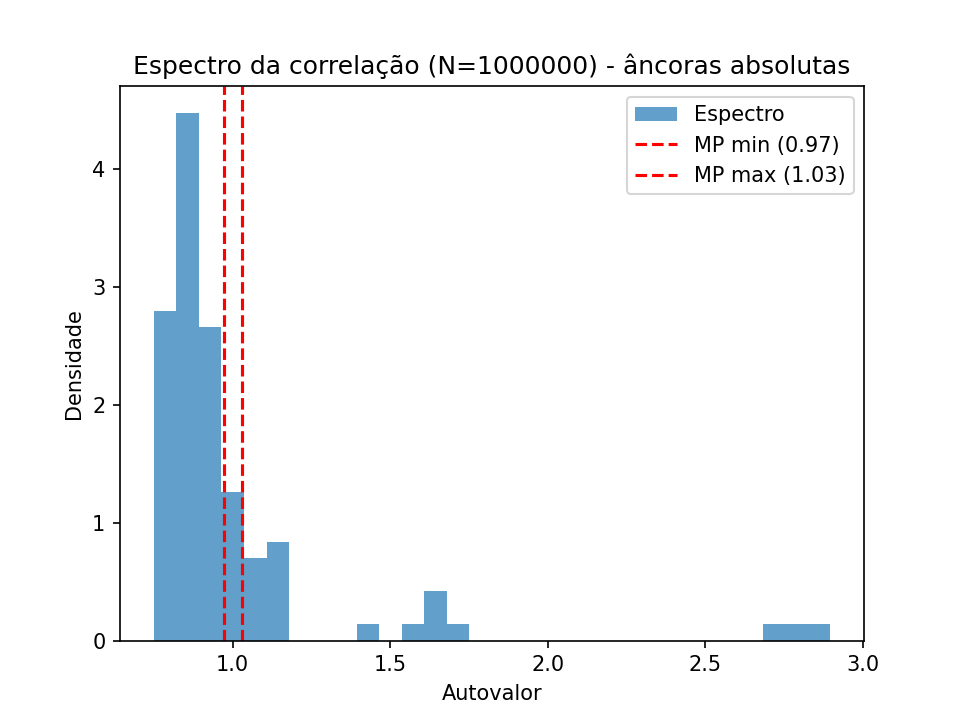
\includegraphics[width=0.45\textwidth]{espectro_N1000000.png}
	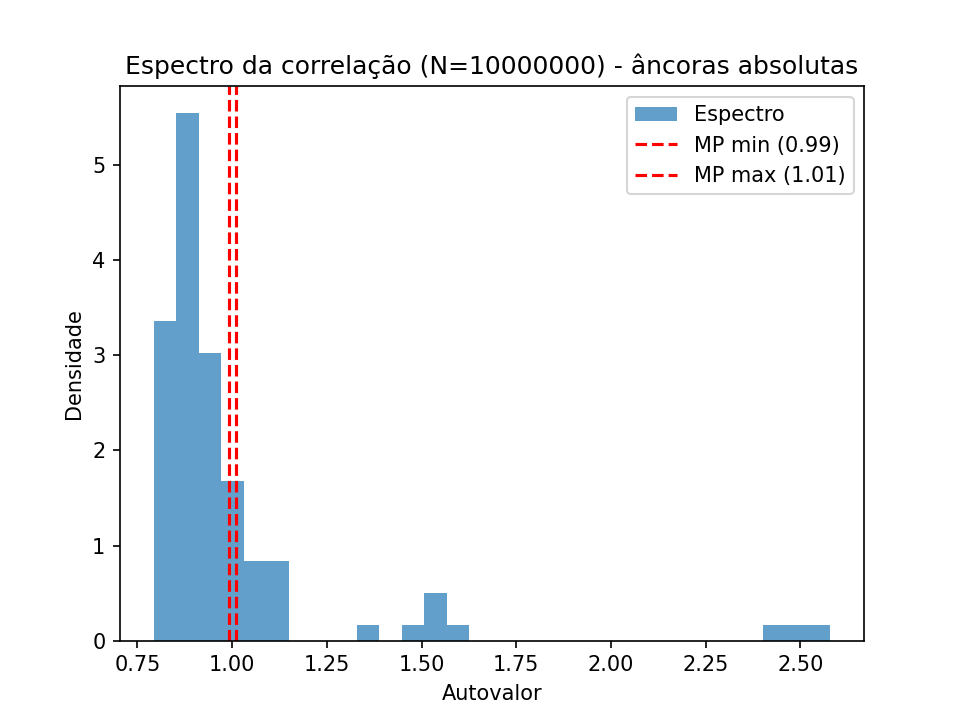
\includegraphics[width=0.45\textwidth]{espectro_N10000000.png}
	\caption{Histograma dos autovalores da matriz de correlação entre as ativações das 100 primeiras âncoras absolutas para $N=10^6$ (esquerda) e $N=10^7$ (direita). As linhas vermelhas indicam os limites de Marčenko–Pastur para uma matriz aleatória. A concentração dos autovalores perto de $1$ e a cauda moderada confirmam a fraca correlação positiva ($<0,4\%$) observada na Tabela~\ref{tab:corr}.}
	\label{fig:espectros}
\end{figure}

A correlação média é \textbf{positiva e menor que $0{,}4\%$}, decrescente com $N$, o que justifica matematicamente o tratamento das ativações como eventos quase-independentes. O pequeno viés positivo é um efeito de borda das âncoras menores ($p=5,7,11,\dots$), que cobrem muitos $C$ baixos em comum; ele não se concentra nas primeiras âncoras — distribui-se uniformemente por todo o conjunto, como verificado excluindo-se as primeiras 10, 20 e 30 âncoras sem alteração significativa da média. A variância empírica do número de coberturas por $C$ é $25$–$38\%$ superior à predita pela independência, mas a \emph{média} é acertada pelo modelo de Poisson — e é a média que governa a saturação exponencial.

É importante notar que a anticorrelação de $-2{,}5\%$ reportada em análises anteriores pertence ao \textbf{regime restrito} ($p \equiv 3 \pmod 8$), onde as âncoras competem pela mesma classe modular escassa. No regime absoluto — o utilizado em todos os experimentos de cobertura deste artigo — esse efeito desaparece e a independência entre janelas é quase perfeita.
	
	
	\subsection{Herança ativa e autossimilaridade via $T(C)=5C+2$}
	
	A transformação $T(C)=5C+2$ define órbitas aritméticas ao longo das quais a sobrevivência do estado ativo de $HR^-$ excede sistematicamente o patamar esperado por um modelo de probabilidade uniforme \cite{art9}. Avaliadas $50{.}000$ sementes no intervalo $[4,\,480{.}079]$ para $N=10^7$:
	
	\begin{itemize}
		\item \textbf{Geração 0} ($C_0$ ativo em $HR^-$): $10{.}490$ de $40{.}014$ sementes.
		\item \textbf{Geração 1} ($C_1 = T(C_0)$ ativo): $2{.}294$ — taxa de sobrevivência real $21{,}9\%$, contra $6{,}7\%$ esperado sob Poisson ingênuo (desvio de $+227\%$).
		\item \textbf{Geração 2} ($C_2 = T(C_1)$ ativo): $392$ — taxa real $17{,}1\%$, contra $6{,}1\%$ esperado (desvio de $+180\%$).
	\end{itemize}
	
	A ressalva metodológica relevante é que o modelo de Poisson ingênuo assume distribuição uniforme, enquanto a heurística de Hardy-Littlewood para o par $(C,\,5C+2)$ já prevê uma densidade local acima do acaso pela exclusão sistemática de divisores pequenos. O ganho dinâmico líquido atribuível ao operador espectral é portanto menor que o desvio bruto, mas a estabilidade do desvio entre gerações confirma o papel da fita-dobra como \emph{atrator} para a densidade espectral — conectando-se diretamente à análise do operador de Koopman desenvolvida em \cite{art6}.
	
	\subsection{Derivação da constante $A_{\text{abs}}$}
	
	No regime restrito, a densidade de âncoras disponíveis é $1/(4\log x)$; no regime absoluto é $1/\log x$. Para um mesmo número de janelas $k^*$, a relação entre os $p_{\max}$ é aproximadamente $\varphi(8)=4$. Usando o valor empírico $A_{\text{restrita}} \approx 44$ para $N=10^7$, obtemos $A_{\text{abs,teórico}} \approx 44/4 = 11$, próximo do observado $10{,}02$. A pequena diferença residual ($\approx 10\%$) é consistente com o efeito de borda das âncoras pequenas — que cobrem uma fração ligeiramente maior de $C$ do que a densidade assintótica prediz — e com a correlação positiva residual de $0{,}3\%$ entre as ativações no regime absoluto.
	
	\section{Conexão com a Reformulação Espectral (Artigo 6)}
	
	O Artigo 6 \cite{art6} introduz o espaço de estados $X_N = \{1,\dots,N-1\}$, a medida uniforme $\mu_N$ e a transformação $T(t)=t+1\pmod{N-1}$. A função de colisão $F(t)=\mathbf{1}_{\mathbb{P}}(E_1(t))\mathbf{1}_{\mathbb{P}}(E_2(t))$ tem transformada de Fourier:
	\[
	\widehat{F}(j) = \frac{1}{N-1}\sum_{t=1}^{N-1} F(t) e^{-2\pi i j t/(N-1)}.
	\]
	A condição $HR^-$ equivale a $\widehat{F}(0) > 0$. O teorema de Green–Tao–Ziegler \cite{GTZ} implica que, para todo $j\neq 0$, $\widehat{F}(j) \to 0$ quando $N\to\infty$: as componentes não nulas são assintoticamente descorrelacionadas.
	
	Os experimentos deste artigo mostram que, para todo $N\le 10^8$, $\sum_t F(t) \ge 1$, logo $\widehat{F}(0) \ge 1/(N-1) > 0$. Portanto, os dados são compatíveis com a predição de que a única barreira espectral é a positividade da frequência zero, e que as demais frequências não contribuem para a existência de pares de Goldbach. Este é um forte indício de que a obstrução analítica identificada em \cite{art6} é de fato a única relevante.
	
	\section{Discussão e Trabalhos Futuros}
	
	\subsection{Comparação com a literatura}
	
	Os resultados conhecidos (Chen, 1966 \cite{chen}) garantem que todo par suficientemente grande é soma de um primo e um semiprimo, sem controle sobre o menor termo. Sob a Hipótese de Riemann Generalizada, sabe-se que o menor primo em uma representação de Goldbach é $O(M^{0,525})$ \cite{BHP}. A Conjectura da Âncora Absoluta propõe um limite \textbf{polilogarítmico}, muito mais forte, mas consistente com a evidência empírica até $10^8$.
	
	\subsection{Lacunas e próximos passos}
	
	A principal lacuna é a prova analítica de que $\widehat{F}(0) > 0$ para todo $N$. A abordagem espectral reduz o problema a estimar a média orbital de $F$, o que pode ser atacado com métodos de crivo mais sofisticados ou com técnicas de recorrência de Furstenberg. Propomos como trabalhos futuros imediatos:
	
	\begin{enumerate}
		\item \textbf{Extensão computacional} até $N=10^9$ para verificar a estabilização de $A_{\text{abs}}$.
		\item \textbf{Análise dos resíduos teimosos}: identificar se os últimos $C$ a serem cobertos pertencem a classes modulares específicas.
		\item \textbf{Refino do modelo de Poisson} incorporando a correlação positiva de $+0{,}3\%$ para corrigir a subestimação da variância ($25$–$38\%$) sem comprometer a predição da média.
		\item \textbf{Tentativa de prova condicional} sob a Hipótese de Riemann Generalizada, usando a estimativa de Siegel–Walfisz para controlar os erros do crivo.
	\end{enumerate}
	
	\section{Conclusão}
	
	O Motor de Herança Estrutural, operando sob a Regra Absoluta, exibe leis de escala claras e robustas: o número de âncoras necessárias para cobrir todos os números pares até $N$ cresce como $5,5\log N$, e o maior primo utilizado cresce como $10,3 \log N \log\log N$. Esses resultados, obtidos por simulação exaustiva até $10^8$, sustentam a \textbf{Conjectura da Âncora Absoluta}: a decomposição de Goldbach pode sempre ser feita com um primo logaritmicamente pequeno. A compatibilidade com a reformulação espectral do Artigo 6 indica que a componente de frequência zero da função de colisão é positiva e que as demais frequências são irrelevantes. Este artigo fecha o ciclo experimental da série, fornecendo uma base quantitativa para a Hipótese Restritiva Fraca e abrindo caminho para futuras investigações analíticas.
	
	\section*{Agradecimentos}
	O autor agradece ao ambiente de desenvolvimento de código aberto que tornou possíveis as simulações extensivas. Os scripts e dados estão disponíveis em \url{https://github.com/tiagobandeira/goldbach-motor}.
	
	\bibliographystyle{plain}
	\begin{thebibliography}{99}
		
		\bibitem{art1} T. Bandeira, \emph{Uma Abordagem Unificada para a Conjectura de Goldbach: Estrutura Combinatória, Saturação Geométrica e o Elo entre Trios e Pares Primos}, preprint (2026).
		\bibitem{art2} T. Bandeira, \emph{Uma Propriedade de Soma Constante na Grade $3\times N$ e as Conjecturas de Goldbach}, preprint (2026).
		\bibitem{art3} T. Bandeira, \emph{O Invariante Âncora da Grade $G_{3,N}$ e um Estimador Geométrico Oracle-Free para a Conjectura de Goldbach}, preprint (2026).
		\bibitem{art4} T. Bandeira, \emph{Problema B do Crivo Geométrico: Demonstração da Desigualdade Estrutural}, preprint (2026).
		\bibitem{art5} T. Bandeira, \emph{Motor de Herança Estrutural: Formalização Algébrica da Fita-Dobra e do Mecanismo de Promoção de Pares de Goldbach}, preprint (2026).
		\bibitem{art6} T. Bandeira, \emph{Reformulação Espectral do Motor de Herança Estrutural: Uma Abordagem por Sistemas Dinâmicos à Conjectura de Goldbach}, preprint (2026).
		\bibitem{art7} T. Bandeira, \emph{Motor de Herança Estrutural: Formalização Definitiva da Fita-Dobra, da Grade Zigzag, da Janela $W_i$ com Quatro Eixos e do Mecanismo de Pivôs}, preprint (2026).
		\bibitem{art8} T. Bandeira, \emph{Operador de Transferência Orbital e Análise Indutiva}, preprint (2026).
		\bibitem{art9} T. Bandeira, \emph{Nota sobre Cadeias de Autossimilaridade e a Transformação $T(C)=5C+2$}, preprint (2026).
		
		\bibitem{GTZ} B. Green, T. Tao, T. Ziegler, \emph{An inverse theorem for the Gowers $U^{s+1}[N]$-norm}, Annals of Mathematics \textbf{176}, 1231–1372 (2012).
		\bibitem{chen} J. R. Chen, \emph{On the representation of a large even integer as the sum of a prime and the product of at most two primes}, Scientia Sinica \textbf{16}, 157–176 (1973).
		\bibitem{BHP} R. C. Baker, G. Harman, J. Pintz, \emph{The difference between consecutive primes, II}, Proceedings of the London Mathematical Society \textbf{83}(3), 532–562 (2001).
		
	\end{thebibliography}
	
\end{document}